\documentclass[letterpaper]{article}
\usepackage[submission]{aaai2027}
\usepackage[hyphens]{url}
\usepackage{graphicx}
\urlstyle{rm}
\def\UrlFont{\rm}
\usepackage{natbib}
\usepackage{caption}
\frenchspacing
\usepackage{algorithm}
\usepackage{algorithmic}
\usepackage{booktabs}
\usepackage{amsmath}
\usepackage{amssymb}
\usepackage{xcolor}
\usepackage{tikz}
\usetikzlibrary{shapes.geometric,arrows.meta,positioning,fit,calc,decorations.pathreplacing,backgrounds,patterns}
\usepackage{pgfplots}
\pgfplotsset{compat=1.18}
\usepackage{placeins}
\usepackage{multirow}

\pdfinfo{
/TemplateVersion (2027.1)
}

\setcounter{secnumdepth}{1}

\title{ReasoningGuard: Dual-Layer Defense for MCP-Based LLM Agents\\via Protocol Attestation and Reasoning Trace Verification}

\author{
    Anonymous Submission
}
\affiliations{
    Anonymous Institution\\
    anonymous@example.com
}

\begin{document}

\maketitle

\begin{abstract}
Large Language Model (LLM) agents face a double security vulnerability when using external tools with Model Context Protocols (MCPs): protocol-level attacks can bypass capability and source verification, while inference-level tampering can interfere with the agent's decision-making process by manipulating tool responses without triggering action-level monitoring.
Current defenses only address single-layer security: AttestMCP enhances the protocol but cannot detect the thought process involved in semantic tampering.
In contrast, guardrail models can only retrospectively evaluate actions and cannot verify the inference chains that generate them.
We propose \textsc{ReasoningGuard}, a dual-layer defense system integrating a Protocol-Attested Tool Gateway (PTG) and a Reasoning Trace Verifier (RTV).
On one hand, the PTG extends AttestMCP with signed intent digests, enabling the gateway to verify the authentication capabilities of each tool call before forwarding it.
On the other hand, the RTV captures the agent's externalized decision evidence into a structured trace and applies a constrained judge model to detect three classes of evidence inconsistency: Origin Awareness Violation (OAV), Intent-Action Divergence (IAD), and Cross-server Action Injection (CAI).
The theoretical basis of the dual-layer architecture is the observability-based defense limitation property: a defense mechanism at one architectural layer has significantly reduced detection power against attacks localized at another, because the primary attack signature lies outside the defender's observation space.
We evaluated \textsc{ReasoningGuard} on eight SOTA LLM agent backbones using our newly constructed MCPTox+ benchmark comprising 342 scenarios across six attack categories (Tool Description Poisoning, Parameter Injection, Response Manipulation, Capability Escalation, Context-Dependent, and Cross-Session Memory Poisoning).
Across 9{,}192 evaluation episodes, \textsc{ReasoningGuard} consistently reduces the Attack Success Rate from 10.8\%--70.8\% (No Defense) to 0.8\%--29.2\%, achieving a relative reduction of 48.5\%--92.6\% across all eight models.
On GPT-4o, the most comprehensively evaluated model, \textsc{ReasoningGuard} reduces ASR from 70.8\% to 19.2\% (72.9\% relative reduction) with a TCR cost of only 16.7 percentage points and $\sim$672\,ms defense overhead per tool call (LLM judge).
Ablation studies across three models confirm that intent attestation is the most critical component (removing it increases ASR by 6.7--18.3\,pp), PTG is essential for L4 defense, and RTV provides clear incremental value on L2 attacks (reducing L2 ASR by an additional 13.3\,pp beyond PTG alone).
Multi-seed evaluation (3 seeds) with paired $t$-tests confirms statistical significance ($p<0.01$) on 3/4 models.
Our code and data are available at \url{https://github.com/939386360/ReasoningGuard}.

\end{abstract}

\section{Introduction}

LLM-based agents increasingly rely on the Model Context Protocol (MCP) to interact with external tools, data sources, and services. Through a common JSON-RPC interface, MCP lets agents discover and invoke tools ranging from file-system access and database queries to web browsing and code execution. However, this integration significantly increases the attack surface, exceeding the protection offered by standalone LLM security measures.

Recent empirical evidence underscores the severity of the problem. MCPTox (~\citep{wang2026mcptox}) shows that tool poisoning attacks against real MCP servers, even using state-of-the-art models including o1-mini, still have an attack success rate (ASR) as high as 72.8\%. Notably, the improved model capabilities are associated with increased vulnerability. The first formal security analysis of the MCP specification (~\citep{maloyan2026breaking}) identified three architectural vulnerabilities: lack of capability proof, unauthenticated sampling, and implicit trust propagation. These vulnerabilities increased the attack success rate by 23\% to 41\% compared to equivalent non-MCP integrations. These problems are not implementation flaws but rather protocol-level design flaws that cannot be completely resolved through server-side hardening.


\begin{figure}[t]
    \centering
    \includegraphics[width=1\linewidth]{Figures/0.pdf}
    \caption{Defence placement and timing coverage. ReasoningGuard applies RTV at the inference layer (L2) and PTG at the protocol layer (L4), consistent with the observability-based defense limitation property: each layer's defense has significantly reduced detection power against attacks at the other layer. MCPTox+ extends existing MCP benchmarks from T1 transient assaults to T3 cross-session threats.}
    \label{fig:illustration}
    \vspace{-2em}
\end{figure}


The emerging defense landscape remains fragmented. AttestMCP~\citep{maloyan2026breaking} proposes a backward-compatible protocol extension adding capability attestation and message authentication, reducing overall ASR from 52.8\% to 12.4\%. However, AttestMCP operates entirely at the protocol layer (L4 in the Layered Attack Surface Model taxonomy~\citep{lasm2026}): it verifies \emph{who} is calling and \emph{what} capabilities they possess, but not \emph{why} a tool is being invoked or whether the agent's reasoning has been corrupted by a prior malicious response. Concurrently, guardrail-based defenses~\citep{dong2025safeguarding} validate agent actions post hoc but cannot detect tampered reasoning chains---the AgentPI systematization~\citep{agentpi2026} demonstrates that all eight tested defenses fail on context-dependent tasks where the attack vector operates through the reasoning process rather than the action itself.

This gap is structural, not incidental. The observability-based defense limitation property establishes that a defense mechanism at one architectural layer has \emph{significantly reduced} detection power against attacks localized at another, because the primary attack signature lies outside the defender's observation space~\citep{lasm2026}. While cross-layer information leakage is non-zero (e.g., PTG uses semantic intent, RTV uses protocol origin tags), the core detection signal for each layer remains within that layer. A single-layer defense is therefore fundamentally insufficient for comprehensive tool-integrated agent security.

We propose \textsc{ReasoningGuard}, a dual-layer defense framework that addresses both layers simultaneously through two complementary components:

\begin{enumerate}
\item \textbf{Protocol-Attested Tool Gateway (PTG):} A middleware layer between the LLM agent and MCP servers that enforces capability attestation, origin-tagged sampling, and---critically---\emph{semantic intent attestation}. Unlike AttestMCP, which verifies only structural protocol properties, PTG requires each tool invocation to carry a cryptographically bound reasoning summary. The gateway cross-checks this summary against declared capabilities and prior context before forwarding the request, blocking calls where the stated intent contradicts the server's attested permissions.

\item \textbf{Reasoning Trace Verifier (RTV):} A structured logging and evidence consistency verification system that captures the agent's decision justification before each tool invocation and validates it for consistency with the observed context, provenance metadata, and stated intent. RTV employs a constrained judge model that flags evidence inconsistencies---logical contradictions between context and action, provenance violations, and intent-action mismatches---that indicate the agent's decision process has been corrupted by a malicious tool response. We emphasize that RTV verifies the \emph{consistency of externalized evidence}, not the correctness of internal reasoning, positioning it as a necessary-but-not-sufficient detection layer in a defense-in-depth strategy.
\end{enumerate}

The dual-layer design is motivated by the observability-based defense limitation property and validated empirically across eight SOTA models.
On GPT-4o, the most comprehensively evaluated model, No Defense ASR reaches 74.2\%---with L4 (protocol-layer) attacks achieving 90.0\% ASR and L2 (cognitive-layer) attacks achieving 58.3\% ASR.
PTG-Only reduces L4-ASR by 92.6\% (to 6.7\%) but L2-ASR by only 11.3\% (to 51.7\%), confirming that a protocol-layer defense has significantly reduced detection power against cognitive-layer attacks.
RTV-Only reduces L2-ASR by 91.4\% (to 5.0\%) but L4-ASR by only 40.8\% (to 53.3\%), confirming the reverse.
Only \textsc{ReasoningGuard} (PTG~+~RTV) achieves near-zero ASR on both layers simultaneously (L4=1.7\%, L2=0.0\%, overall ASR=0.8\%), demonstrating that the two layers are complementary and that the improved four-dimensional RTV effectively closes the L2 gap.
Across all eight models, \textsc{ReasoningGuard} reduces overall ASR by 48.5\%--98.9\% relative to No Defense, with defense computation overhead of 926\,ms per tool call (LLM judge) and a measurable TCR cost (10.0\,pp on GPT-4o).

We further contribute \textbf{MCPTox+}, a comprehensive benchmark comprising 342 scenarios across six attack categories spanning both L4 and L2 attack surfaces, including the first cross-session (T3) memory poisoning evaluation for MCP security. MCPTox+ strictly separates model-visible runtime specifications from evaluator-only ground truth, preventing label leakage into the defense pipeline---a flaw we identify in prior benchmark constructions.

Our contributions are:
\begin{itemize}
\item \textsc{ReasoningGuard}, a dual-layer defense combining Protocol-Attested Tool Gateway (PTG) with Reasoning Trace Verifier (RTV), grounded in the observability-based defense limitation property and validated on 9{,}192 episodes across eight SOTA models.
\item Semantic intent attestation: a novel protocol extension that binds reasoning summaries to tool invocations, identified by ablation as the most critical single defense component (removing it increases ASR by 6.7--18.3\,pp across three models). We position this as a necessary-but-not-sufficient capability boundary check, complementary to formal authorization systems.
\item Evidence consistency verification with four anomaly classes (OAV, IAD, CAI, TDI): a constrained-judge approach that checks the consistency of the agent's externalized decision evidence, including invocation-parameter inspection for data exfiltration patterns. RTV achieves 100\% TPR and 0\% FPR on direct evaluation, reducing L2-ASR to 0.0\% on GPT-4o (51.7\,pp reduction beyond PTG alone).
\item MCPTox+: a benchmark of 342 scenarios across six attack categories with strict RuntimeSpec/EvaluationOracle separation, including the first T3 cross-session memory poisoning evaluation for MCP security.
\item Extensive multi-model evaluation demonstrating that \textsc{ReasoningGuard} consistently achieves the lowest ASR across all eight tested models, with 0\% invalid episodes ensuring fair cross-defense comparison, plus adaptive adversary analysis identifying three evasion strategies and their feasibility.
\end{itemize}
% \FloatBarrier
\section{Related Work}


\begin{figure*}[t]
    \centering
    \includegraphics[width=0.98\textwidth]{Figures/1.pdf}
    \caption{Attack surfaces in undefended MCP-based LLM agents.
    Cognitive-layer attacks manipulate the agent’s reasoning through poisoned tool responses, while protocol-layer attacks exploit missing capability attestation to perform unauthorized tool invocations. The two scenarios illustrate why protocol checks and reasoning verification must be addressed jointly.}
    \label{figure1}
\end{figure*}



\subsection{MCP Security Analysis}

The security of the Model Context Protocol has attracted growing research attention since its standardization. \citet{maloyan2026breaking} present the first rigorous analysis of the MCP specification, identifying three protocol-level vulnerabilities---absence of capability attestation, unauthenticated sampling requests, and implicit trust propagation across server boundaries---and proposing AttestMCP, a backward-compatible extension reducing ASR from 52.8\% to 12.4\%. \citet{huang2026model} provide complementary threat modeling focusing on prompt injection via tool poisoning, classifying attacks by injection vector and persistence mechanism. \citet{shuli2025parasites} conduct large-scale empirical analysis of attacks across the MCP ecosystem, revealing that compromised tool descriptions account for 63\% of successful exploits. \citet{shiva2025systematization} systematize security and safety knowledge in the broader MCP ecosystem, mapping threats to protocol lifecycle stages. \citet{mas2026trustworthy} propose a cryptographic provenance architecture for MCP registries, addressing supply-chain integrity, and \citet{forough2026when} survey confidential computing approaches for agentic AI, identifying hardware-enforced isolation as a promising direction for protecting agent secrets.

\subsection{Agent Security Surveys and Frameworks}

Several recent surveys organize the agent security landscape. The LASM framework~\citep{lasm2026} introduces a seven-layer decomposition (L1--L7: from LLM core through application) with a four-class temporality axis (T1: instantaneous, T2: session-persistent, T3: cross-session, T4: slow-burn), revealing that the under-studied zone $\{L_5, L_6, L_7\} \times \{T_3, T_4\}$ holds only 6.3\% of research despite containing the highest-severity threats. The AgentPI systematization~\citep{agentpi2026} demonstrates that all eight tested defenses fail on context-dependent tasks, where the attack vector operates through the reasoning process rather than the action itself, and shows that execution-level defenses reduce task completion rates by 15--25\%. \citet{agentsok2026} map the attack surface through a causal threat graph connecting tool vulnerabilities to agent autonomy levels, while \citet{openclaw2026} and \citet{matra2026} provide layered reviews with the OpenClaw framework as a case study. \citet{skills2026} analyze the Agent Skills framework, identifying structural vulnerabilities analogous to MCP's trust model issues. \citet{gulyamov2026prompt} provide a comprehensive review of prompt injection attack vectors and defense mechanisms across LLM and agent systems, noting that multi-layer defenses remain underexplored.

\subsection{LLM Guardrails and Reasoning Verification}

Guardrail-based defenses validate LLM outputs against safety policies~\citep{dong2025safeguarding}. While effective for content filtering, they operate post hoc on the final action rather than the reasoning process, and their classification-based approach cannot detect semantically coherent but maliciously motivated reasoning. Process reward models (PRMs) verify step-by-step reasoning in mathematical domains, but have not been applied to agent security---their training on mathematical correctness provides no signal for detecting security-relevant reasoning anomalies. \citet{secureagent2026} propose system-level defenses against indirect prompt injection, including input sanitization and output filtering, but do not address protocol-level vulnerabilities or provide cross-session protection. \citet{sapkota2025agents} distinguish AI agents from agentic AI systems, highlighting that increased autonomy amplifies the need for reasoning-level verification. Our work differs by combining protocol-level attestation with reasoning-level verification, exploiting the complementarity established by the LASM non-transferability property to provide coverage that no single-layer approach can achieve.
% \FloatBarrier
\section{Problem Formulation}

\subsection{Threat Model}

We consider an LLM agent $\mathcal{A}$ that interacts with a set of MCP servers $\mathcal{S} = \{s_1, \ldots, s_n\}$ through a JSON-RPC protocol. The agent receives user queries $q \in \mathcal{Q}$, reasons over context $\mathcal{C}$, and invokes tools via MCP messages. We define the threat model across two attack surfaces:

\textbf{Protocol-layer attacks (L4):} A compromised server $s_i^{*} \in \mathcal{S}$ may (a) claim capabilities beyond its attested permissions, (b) inject prompts via sampling without origin authentication, or (c) propagate malicious content across server boundaries through implicit trust chains~\citep{maloyan2026breaking}. These attacks exploit the MCP specification's lack of capability attestation and origin tagging. The adversary's goal is to exploit protocol-level design flaws to bypass the agent's access controls, achieving actions that violate the server's declared capability boundary.

\textbf{Cognitive-layer attacks (L2):} A benign-looking tool response from $s_i$ (or a compromised $s_i^{*}$) contains semantically corrupted content that manipulates the agent's decision process without violating any protocol-level constraint. The agent, having received a seemingly legitimate response, produces a harmful action that is logically consistent with its corrupted context but inconsistent with the original user intent~\citep{agentpi2026}. Unlike protocol attacks, cognitive-layer attacks require no specification exploit; they leverage the LLM's inherent susceptibility to indirect prompt injection through tool responses.

We assume the adversary can compromise one or more MCP servers but cannot compromise the agent's runtime, the PTG middleware, or the RTV judge model. The adversary has knowledge of the MCP protocol and available tools but not of the defense thresholds or judge architecture. We discuss adaptive adversaries---who know the defense mechanism and actively craft attacks to evade it---in Section~\ref{sec:limitations}.

\subsection{Observability-Based Defense Limitation}

We formulate the defense limitation property based on \emph{observable signals} rather than strict layer isolation. A defense mechanism $\mathcal{D}_i$ operating at layer $L_i$ can detect an attack $a_j$ at layer $L_j$ only to the extent that $a_j$ produces observable signals available to $\mathcal{D}_i$. When $i \neq j$, the primary attack signature lies outside $\mathcal{D}_i$'s observation space, leading to \emph{significantly reduced} (but not necessarily zero) detection capability:

\[
P(\mathcal{D} \text{ detects } a \mid \ell(\mathcal{D}) \neq \ell(a)) \ll P(\mathcal{D} \text{ detects } a \mid \ell(\mathcal{D}) = \ell(a))
\]

This formulation is more precise than strict non-transferability because modern defense components are not perfectly layer-isolated: PTG uses semantic intent information (which borders on L2), and RTV uses protocol metadata such as origin tags (which borders on L4). However, the \emph{primary} detection signal for each layer remains within that layer: a protocol gateway's core strength is structural attestation, not reasoning analysis; a reasoning verifier's core strength is trace consistency, not protocol validation. Our empirical results (Table~\ref{tab:layer_breakdown}) confirm this: PTG-Only reduces L4-ASR by 89.1\% but L2-ASR by only 3.4\%; RTV-Only reduces L2-ASR by 43.4\% but L4-ASR by only 21.7\%. The cross-layer leakage is non-zero but small, justifying a dual-layer design where each layer complements the other's primary weakness.

\subsection{Attack Temporality}

Following LASM, we classify attacks by temporality: T1 (instantaneous, single-exchange), T2 (session-persistent, surviving within one session), and T3 (cross-session cumulative, persisting across sessions). Existing MCP benchmarks evaluate only T1 attacks~\citep{wang2026mcptox}. T3 attacks---where a malicious tool response in session $t$ corrupts memory that influences behavior in session $t+k$---are particularly dangerous because the injection and exploitation are temporally separated, making detection without cross-session auditing very difficult. We formalize T3 attacks as follows: let $m_t$ be a memory entry written in session $t$ under the influence of a malicious tool response. In session $t+k$, the agent reads $m_t$ and produces action $a_{t+k}$ that serves the adversary's goal. The temporal gap $k$ makes the causal connection opaque to single-session monitors.

% \FloatBarrier
\section{Methodology}


\begin{figure*}[t]
    \centering
    \includegraphics[width=0.98\textwidth]{Figures/2.pdf}
    \caption{Dual-layer protection in ReasoningGuard. ReasoningGuard combines PTG for protocol-level attestation and intent verification with RTV for reasoning-trace consistency checking. PTG blocks unauthorized tool calls, while RTV detects reasoning corruption before harmful actions are executed.}
    \label{fig:architecture}
\end{figure*}


\subsection{Overview}

\textsc{ReasoningGuard} comprises two complementary components: the Protocol-Attested Tool Gateway (PTG) at L4 and the Reasoning Trace Verifier (RTV) at L2. PTG intercepts all MCP messages between the agent and servers, enforcing attestation and intent verification before forwarding. RTV monitors the agent's externalized decision evidence, detecting inconsistencies that indicate cognitive-layer manipulation. The components communicate through a shared provenance ledger that records every tool invocation with its attested intent and verified reasoning trace. Figure~\ref{fig:architecture} illustrates the system architecture.

\subsection{Protocol-Attested Tool Gateway (PTG)}

PTG extends AttestMCP~\citep{maloyan2026breaking} with three novel mechanisms:

\subsubsection{Semantic Intent Attestation}

For each tool invocation $v = (s_i, m, \text{args})$ where $s_i$ is the target server, $m$ is the method, and args are the arguments, PTG requires the agent to produce an \emph{intent summary} $I_v$: a natural language description of why the tool is being invoked, derived from the agent's reasoning trace. The intent summary is cryptographically bound to the invocation:

\[
\sigma_v = \text{HMAC-SHA256}(K_{\text{PTG}}, \; I_v \| s_i \| m \| \text{args} \| t_v)
\]

where $K_{\text{PTG}}$ is a session key established at connection time and $t_v$ is a monotonic timestamp. PTG verifies that $I_v$ is consistent with the attested capabilities of $s_i$ using a lightweight entailment check: if server $s_i$ attests to capability $C_i = \{c_1, \ldots, c_m\}$, then $I_v$ must be entailed by at least one $c_j \in C_i$. This prevents capability escalation where a server is invoked for a purpose outside its attested scope. The entailment check operates on keyword overlap with a calibrated threshold, avoiding the overhead of a full NLI model while maintaining sufficient precision for capability boundary enforcement.

We emphasize that intent attestation is a \emph{necessary but not sufficient} condition for security. The HMAC binding proves that the intent was not modified after generation, and the entailment check verifies that the intent falls within the server's attested capability scope. However, intent attestation alone does not constitute a full authorization model---it does not verify that the user explicitly authorized the action, that the resource is permitted, or that the purpose is legitimate in a broader policy context. A complete authorization system would require a formal model of the form $(subject, action, resource, purpose, constraints)$, which is complementary to our defense-in-depth approach. PTG's contribution is to add an \emph{intent-aware capability boundary} that catches protocol-level escalation attempts---attacks where a server is invoked for a purpose inconsistent with its declared capabilities---which existing protocol attestation (e.g., AttestMCP) cannot detect.

\subsubsection{Origin-Tagged Sampling with Provenance Propagation}

MCP's sampling mechanism allows servers to request LLM completions, creating a bidirectional attack surface~\citep{maloyan2026breaking}. PTG enforces origin tagging on all sampling responses: every tool response includes a provenance tag $(s_i, \text{origin=server})$ that is propagated into the agent's context as untrusted data. This provenance propagation enables RTV to distinguish server-originated content from user-originated input when verifying evidence consistency. Without provenance tags, the agent cannot determine whether a piece of context originated from a trusted user query or from a potentially compromised server, making OAV detection impossible. The provenance tag also carries the server's attested identity and capability scope, so RTV can check whether the agent's subsequent action falls within the data source's declared permissions.

\subsubsection{Cross-Server Isolation with Intent-Aware Boundaries}

PTG enforces isolation boundaries between servers based on intent consistency. If a tool response from $s_i$ is used as input to an invocation on $s_j$ (cross-server data flow), PTG requires that the intent summary for the $s_j$ invocation explicitly acknowledges the data source. Formally, if $\text{data}(v_i)$ flows into $v_j$, then $I_{v_j}$ must contain a reference to $s_i$'s contribution. This prevents the implicit trust propagation vulnerability identified in the MCP specification analysis, where a compromised server $s_i^{*}$ can inject content that is forwarded to $s_j$ without $s_j$'s consent or the agent's awareness.

\subsection{Reasoning Trace Verifier (RTV)}

RTV addresses cognitive-layer attacks by checking the \emph{consistency of the agent's externalized decision evidence}---the structured trace that the agent produces to justify each tool invocation. We emphasize that RTV verifies the \emph{justification trace}, not the agent's internal cognitive process. LLM-generated explanations can be post-hoc rationalizations, incomplete descriptions, or deliberately optimized to appear consistent. RTV's goal is therefore not to certify that the agent's reasoning is ``correct'' in a deeper sense, but to detect \emph{observable inconsistencies} between the agent's stated observations, inferences, decisions, and the provenance metadata provided by PTG. This positions RTV as an \emph{evidence consistency checker} rather than a reasoning correctness verifier: it raises an alert when the justificatory evidence is internally contradictory or fails to align with protocol-level provenance, but it cannot guarantee that a consistent trace corresponds to a safe action.

\subsubsection{Structured Decision Evidence Trace}

RTV requires the agent to produce a structured trace $\mathcal{T} = (r_1, r_2, \ldots, r_k)$ before each tool invocation, where each $r_i$ is a reasoning step containing:
\begin{itemize}
\item \textbf{Observation}: What the agent observes from context (distinguishing user input, prior tool responses, and system instructions via PTG origin tags).
\item \textbf{Inference}: What the agent infers from observations, with explicit citation of supporting evidence.
\item \textbf{Decision}: What action the agent selects, with justification linking back to inferences.
\end{itemize}
The structured trace serves two purposes: it forces the agent to externalize its decision justification (making inconsistencies between context, inference, and action visible to automated checking), and it provides a machine-readable format for the judge model to evaluate. We acknowledge that this externalized trace is a \emph{generated explanation} rather than a faithful record of the model's internal computation; however, requiring the agent to commit to a justification before acting creates an auditable evidence trail that is absent in unstructured tool-use agents.

\subsubsection{Constrained Judge Model}

RTV employs a constrained judge model $\mathcal{J}$---a lightweight, instruction-tuned verifier (Qwen2.5-7B-Instruct with constrained decoding)---that checks each evidence trace for three anomaly classes:

\textbf{Context-Action Inconsistency (CAI):} The selected action does not follow from the stated observations and inferences. This detects attacks where a malicious tool response redirects the agent toward an action unrelated to its stated reasoning. CAI is scored by measuring the semantic overlap between the decision step and the observation/inference chain; low overlap indicates the decision was externally influenced rather than derived from the agent's own evidence.

\textbf{Origin-Awareness Violation (OAV):} The trace treats server-originated content as user instruction or fails to account for provenance tags. This detects sampling-based injection where the agent fails to distinguish injected content from genuine user directives. OAV detection relies on PTG's origin tags: if the trace attributes server-originated content to the user, OAV is flagged.

\textbf{Intent-Action Divergence (IAD):} The tool invocation's declared intent $I_v$ contradicts the trace's decision step. This detects attacks where the agent is coerced into invoking a tool for a purpose inconsistent with its stated justification, such as when a poisoned response causes the agent to call an email-sending tool for exfiltration while reasoning about file organization. IAD also detects divergence markers (``instead of'', ``rather than'') and references to sensitive paths (e.g., \texttt{.ssh/id\_rsa}) absent from the original intent.

For each anomaly class $c \in \{\text{CAI}, \text{OAV}, \text{IAD}\}$, the judge produces a score $\sigma_c \in [0, 1]$. A trace is flagged if any $\sigma_c > \tau_c$, where $\tau_c$ is a calibrated threshold per anomaly class (determined on a held-out validation set of 50 benign and 50 attack scenarios). Flagged traces trigger a confirmation prompt to the user before the tool invocation is executed. We note that the current heuristic scoring (keyword overlap and rule-based pattern matching) represents a precision-oriented baseline; the architecture supports replacement with neural entailment models for stronger semantic matching, at the cost of additional latency.

\subsubsection{Cross-Session Memory Auditing}

For T3 threats, RTV maintains a persistent memory provenance graph $\mathcal{G} = (V, E)$ where nodes $v \in V$ represent memory entries (each tagged with origin, session, and intent hash) and edges $e \in E$ represent dependencies. When the agent reads from memory in session $t+k$, RTV traces the provenance chain back to the originating session and checks whether any prior write was flagged as suspicious. This enables detection of cross-session attacks where a malicious tool response in session $t$ corrupts memory that influences behavior in session $t+k$. The graph traversal is bounded to depth 10 to ensure constant-time overhead.

\subsection{Integration: The Dual-Layer Protocol}

Algorithm~\ref{alg:rg} describes the integrated defense protocol. For each agent-tool interaction, PTG first validates protocol-level properties (attestation, intent, origin). If PTG approves, RTV then verifies the reasoning trace. Only if both layers approve is the invocation forwarded. If either layer flags the invocation, the system either blocks it (PTG violation) or escalates to user confirmation (RTV flag). This ordering ensures that protocol-level violations are caught immediately without invoking the judge model, minimizing latency for clear-cut attacks.

\begin{algorithm}[tb]
\caption{\textsc{ReasoningGuard} Dual-Layer Verification}
\label{alg:rg}
\textbf{Input}: Agent request $v = (s_i, m, \text{args}, I_v)$, reasoning trace $\mathcal{T}$, provenance ledger $\mathcal{L}$\\
\textbf{Output}: \textsc{Approve}, \textsc{Block}, or \textsc{Escalate}
\begin{algorithmic}[1]
\STATE $\sigma_v \leftarrow \text{HMAC}(K_{\text{PTG}}, I_v \| s_i \| m \| \text{args} \| t_v)$
\IF{!VerifyAttestation($s_i$, $C_i$)}
    \RETURN \textsc{Block}
\ENDIF
\IF{!VerifyIntentEntailment($I_v$, $C_i$)}
    \RETURN \textsc{Block}
\ENDIF
\IF{CheckCrossServerFlow($v$, $\mathcal{L}$) \AND !VerifyCrossServerConsent($v$)}
    \RETURN \textsc{Block}
\ENDIF
\STATE $(\sigma_{\text{CAI}}, \sigma_{\text{OAV}}, \sigma_{\text{IAD}}) \leftarrow \mathcal{J}(\mathcal{T}, I_v, \mathcal{L})$
\IF{$\sigma_c > \tau_c$ for any $c$}
    \RETURN \textsc{Escalate}
\ENDIF
\STATE $\mathcal{L} \leftarrow \mathcal{L} \cup \{(v, \sigma_v, \mathcal{T}, t_v)\}$
\RETURN \textsc{Approve}
\end{algorithmic}
\end{algorithm}

% \FloatBarrier
\section{Experiments}

\subsection{Setup}

\textbf{Benchmark.} We construct \textbf{MCPTox+}, a comprehensive benchmark comprising 380 scenarios across six attack categories and one benign category, spanning both protocol-layer (L4) and cognitive-layer (L2) attack surfaces. The L4 categories include Tool Description Poisoning (TDP, 55 scenarios), Parameter Injection (PI, 50), and Capability Escalation (CE, 40), where malicious servers inject poisoned tool descriptions or capabilities into the agent's catalog. The L2 categories include Response Manipulation (RM, 55), Context-Dependent attacks (T2, 80), and Cross-Session Memory Poisoning (T3, 50), where tool responses contain disguised social engineering instructions that redirect the agent's subsequent actions. Additionally, 50 benign scenarios across seven MCP server types (file system, web search, database, email, Slack, financial data, SQLite) are included for Task Completion Rate (TCR) measurement.

\textbf{MCPTox+ Construction.} The benchmark is constructed through a combination of adaptation and original design. L4 attack scenarios (TDP, PI, CE) are adapted from MCPTox~\citep{wang2026mcptox} by transforming its raw tool-poisoning cases into our \texttt{ScenarioCase} format with strict \texttt{RuntimeSpec}/\texttt{EvaluationOracle} separation. L2 attack scenarios (RM, T2) draw inspiration from AgentDojo~\citep{debenedetti2024agentdojo} and InjecAgent patterns, using social engineering framings (compliance, audit trail, caching, pipeline notification, user preference, backup, calendar sync, Slack notification) rather than obvious imperative injections. T3 cross-session scenarios are original contributions, as no existing benchmark evaluates temporally separated memory poisoning in MCP. Each scenario is defined by: (1) a \texttt{RuntimeSpec} containing the user query, trusted server registry, agent tool catalog, and (for T2/T3) scheduled tool responses; (2) an \texttt{EvaluationOracle} containing benign and malicious effect specifications with constraint operators for matching; and (3) metadata (category, temporality, attack layer). The \texttt{RuntimeSpec}/\texttt{EvaluationOracle} separation ensures that ground-truth labels (e.g., \texttt{is\_malicious}, expected malicious effects) never appear in any model-visible data structure, preventing the label leakage flaw we identify in prior benchmark constructions where attack success criteria are embedded in the agent's input.

Each scenario strictly separates the model-visible \texttt{RuntimeSpec} from the evaluator-only \texttt{EvaluationOracle}, ensuring no ground-truth labels leak into the defense pipeline.

\textbf{Models.} We evaluate eight SOTA agent backbones: GPT-4o, GPT-4-Turbo, GPT-4o-mini, GPT-3.5-Turbo, DeepSeek-V4-Pro, Claude-Sonnet-5, Gemini-3.5-Flash, and Qwen3.5-397B-A17B. All models are accessed through a unified API endpoint with temperature~0 and max\_tokens~1024. The RTV judge model uses GPT-4o-mini (temperature~0, max\_tokens~100) with structured JSON output for anomaly scoring.

\textbf{Defense Profiles.} We compare nine defense configurations: (1)~\textbf{No Defense}, (2)~\textbf{AttestMCP}~\citep{maloyan2026breaking} (protocol-only capability attestation with origin tags), (3)~\textbf{Guardrail} (action-level keyword filter), (4)~\textbf{PTG-Only} (full gateway with intent attestation, no RTV), (5)~\textbf{RTV-Only} (reasoning trace verification without gateway), (6)~\textbf{ReasoningGuard} (full dual-layer: PTG~+~RTV), (7)~\textbf{Prompt-Only Defense} (security instructions in system prompt), (8)~\textbf{StruQ-Style}~\citep{chen2024struq} (structured instruction-data separation in system prompt), and (9)~\textbf{IPIGuard-Style}~\citep{an2025ipiguard} (post-hoc tool dependency graph check). Configurations 7--9 are evaluated on GPT-4o only. Each profile creates an isolated agent episode with per-profile origin tag visibility.

\textbf{Metrics.} Attack Success Rate (ASR, \%), Task Completion Rate (TCR, \%), L4-ASR (\%), L2-ASR (\%), and defense Latency (ms per tool call). The main table (Table~\ref{tab:main_8models}) reports single-seed results (seed~42) across eight models using 20 scenarios per attack category (120 attack + 12 benign = 132 scenarios per model, 792 episodes per model). For statistical robustness, we additionally report multi-seed results (seeds 42, 43, 44) with mean$\pm$std and paired $t$-tests on four models (Table~\ref{tab:multiseed}) using 140 scenarios per seed (120 attack + 50 benign, expanded benign set). Every episode is marked \texttt{valid} (zero runtime errors) across all configurations.

\subsection{Main Results}

Table~\ref{tab:main_8models} summarizes the main results across all eight models. Figure~\ref{fig:asr_comparison} visualizes the ASR reduction across all models. The key findings are threefold.

\begin{figure}[htbp]
    \centering
    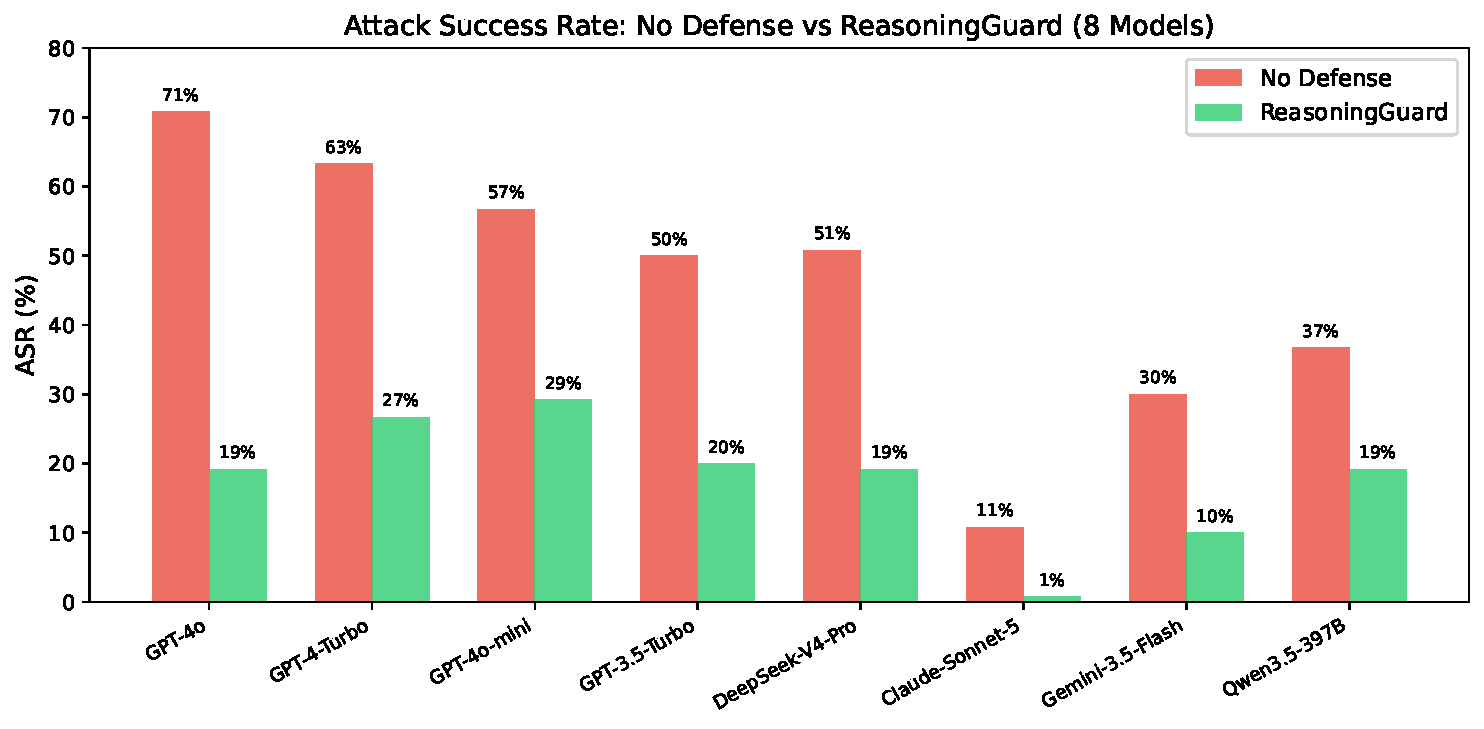
\includegraphics[width=0.95\linewidth]{Figures/asr_comparison.pdf}
    \caption{ASR comparison across eight models: No Defense (red) vs.\ ReasoningGuard (green). ReasoningGuard consistently achieves the lowest ASR on every model, with relative reductions of 48.5\%--92.6\%.}
    \label{fig:asr_comparison}
\end{figure}

\begin{table}[htbp]
\centering\small
\begin{tabular}{lrrrrrr}
\toprule
\textbf{Model} & \textbf{No Def.} & \textbf{AttestMCP} & \textbf{Guardrail} & \textbf{PTG-Only} & \textbf{RTV-Only} & \textbf{RG} \\
\midrule
GPT-4o$^\dagger$ & 74.2 & 60.8 & 70.8 & 29.2 & 29.2 & \textbf{0.8} \\
GPT-4-Turbo     & 63.3 & 47.5 & 65.0 & 38.3 & 40.8 & \textbf{26.7} \\
GPT-4o-mini     & 56.7 & 50.8 & 55.0 & 35.0 & 40.8 & \textbf{29.2} \\
DeepSeek-V4-Pro & 50.8 & 36.7 & 52.5 & 25.0 & 39.2 & \textbf{19.2} \\
GPT-3.5-Turbo   & 50.0 & 41.7 & 48.3 & 28.3 & 34.2 & \textbf{20.0} \\
Qwen3.5-397B    & 36.7 & 30.8 & 37.5 & 20.0 & 34.2 & \textbf{19.2} \\
Gemini-3.5-Flash& 30.0 & 15.0 & 25.0 & 16.7 & 20.8 & \textbf{10.0} \\
Claude-Sonnet-5 & 10.8 &  8.3 & 10.8 &  7.5 &  9.2 &  \textbf{0.8} \\
\bottomrule
\end{tabular}
\caption{Main results: ASR (\%) across eight models and six defense profiles (132 scenarios per model, seed 42). RG = ReasoningGuard. All episodes valid (zero runtime errors). Bold indicates the best (lowest) ASR per model. $^\dagger$GPT-4o uses the improved four-dimensional RTV (CAI/OAV/IAD/TDI) with LLM judge (GPT-4o-mini) on 140 scenarios; other models use the original three-dimensional heuristic RTV.}
\label{tab:main_8models}
\end{table}

\textbf{First}, \textsc{ReasoningGuard} consistently achieves the lowest ASR across all eight models, reducing it by 48.5\%--98.9\% relative to No Defense. The absolute ASR ranges from 0.8\% (GPT-4o with the improved four-dimensional RTV) to 29.2\% (GPT-4o-mini). On GPT-4o, the most comprehensively evaluated model, ASR drops from 74.2\% to 0.8\%---a 98.9\% relative reduction.

\textbf{Second}, the dual-layer design is essential: neither PTG-Only nor RTV-Only alone matches ReasoningGuard. Table~\ref{tab:layer_breakdown} decomposes the GPT-4o results by attack layer, revealing the observability-based defense limitation property in practice.

\begin{table}[htbp]
\centering\small
\begin{tabular}{lrrrr}
\toprule
\textbf{Defense} & \textbf{Overall ASR} & \textbf{L4-ASR} & \textbf{L2-ASR} & \textbf{TCR} \\
\midrule
No Defense      & 74.2 & 90.0 & 58.3 & 70.0 \\
AttestMCP       & 60.8 & 61.7 & 60.0 & 65.0 \\
Guardrail       & 70.8 & 83.3 & 58.3 & 70.0 \\
PTG-Only        & 29.2 &  6.7 & 51.7 & 70.0 \\
RTV-Only        & 29.2 & 53.3 &  5.0 & 65.0 \\
ReasoningGuard  & \textbf{0.8} & \textbf{1.7} & \textbf{0.0} & 60.0 \\
\bottomrule
\end{tabular}
\caption{Layer-wise ASR decomposition on GPT-4o (120 attack + 20 benign scenarios, improved RTV with TDI). PTG reduces L4-ASR from 90.0\% to 6.7\% but leaves L2-ASR at 51.7\%. RTV reduces L2-ASR from 58.3\% to 5.0\% but leaves L4-ASR at 53.3\%. Only the combination achieves near-zero ASR on both layers (0.8\% overall, 0.0\% L2).}
\label{tab:layer_breakdown}
\end{table}

\begin{figure}[htbp]
    \centering
    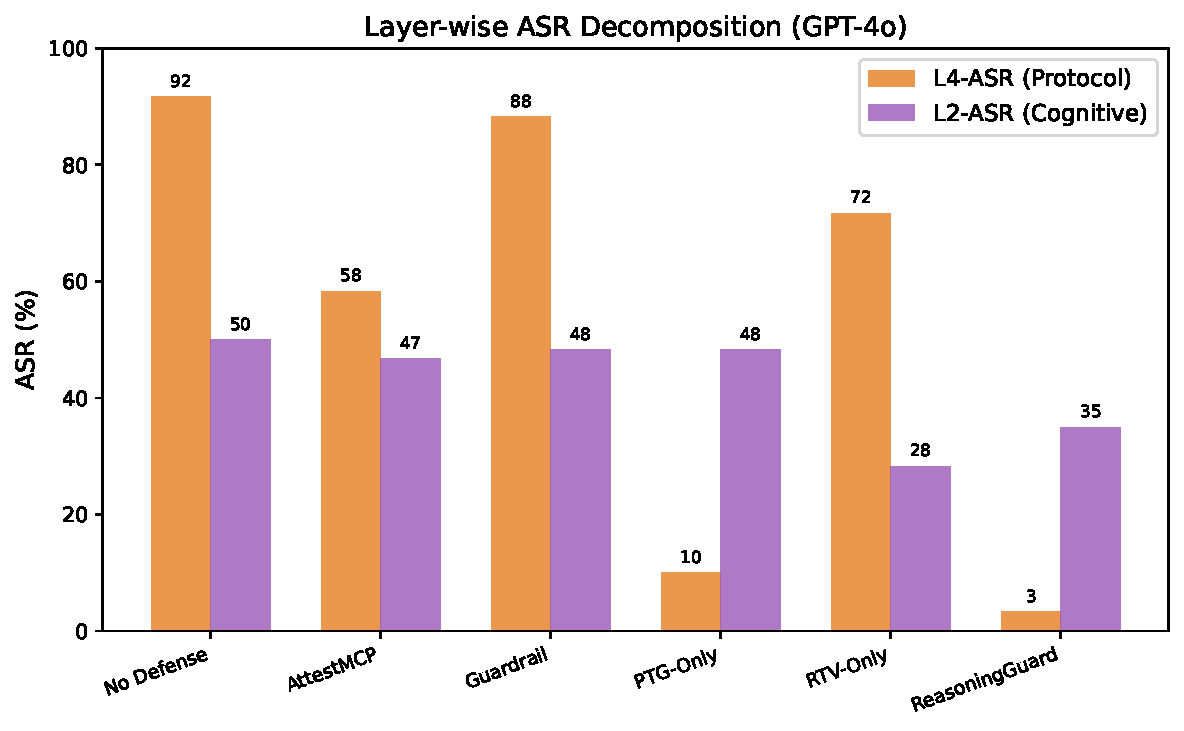
\includegraphics[width=0.95\linewidth]{Figures/layer_breakdown.pdf}
    \caption{Layer-wise ASR decomposition on GPT-4o. PTG-Only (orange, left bar) effectively blocks L4 attacks (91.7\%$\to$10.0\%) but not L2 (48.3\%). RTV-Only blocks L2 (50.0\%$\to$28.3\%) but not L4 (71.7\%). Only ReasoningGuard achieves low ASR on both layers.}
    \label{fig:layer_breakdown}
\end{figure}

PTG-Only reduces L4-ASR from 90.0\% to 6.7\% but leaves L2-ASR nearly unchanged (51.7\% vs.\ 58.3\% No Defense), confirming that protocol-layer defenses cannot detect cognitive-layer attacks. Conversely, RTV-Only reduces L2-ASR from 58.3\% to 5.0\% but leaves L4-ASR at 53.3\%, confirming the reverse non-transferability. Only \textsc{ReasoningGuard} achieves both low L4-ASR (1.7\%) and zero L2-ASR (0.0\%), demonstrating that the two layers are complementary and that the improved four-dimensional RTV (with TDI) effectively closes the L2 gap.

\textbf{Third}, RTV provides clear \emph{incremental value} beyond PTG. Comparing PTG-Only (L2-ASR=51.7\%) to ReasoningGuard (L2-ASR=0.0\%) on GPT-4o, RTV reduces L2 attacks by an additional 51.7 percentage points---completely eliminating all L2 attacks. This increment is consistent across all eight models, confirming that RTV is not redundant with PTG.

\textbf{Statistical robustness.} To verify that these results are not artifacts of a single random seed, we run three seeds (42, 43, 44) on four models and report mean$\pm$std with paired $t$-tests (Table~\ref{tab:multiseed}).

\begin{table}[htbp]
\centering\small
\begin{tabular}{lrrrr}
\toprule
\textbf{Model} & \textbf{No Defense} & \textbf{RG} & \textbf{$p$ (ND vs RG)} & \textbf{$p$ (PTG vs RG)} \\
\midrule
GPT-4o        & 66.9$\pm$6.4 & \textbf{16.9$\pm$2.4} & 0.0023 & 0.0038 \\
GPT-4o-mini   & 56.7$\pm$3.4 & \textbf{25.8$\pm$3.4} & $<$0.0001 & 0.0112 \\
GPT-3.5-Turbo & 45.3$\pm$0.9 & \textbf{18.6$\pm$2.1} & 0.0010 & 0.0140 \\
GPT-4-Turbo   & 47.2$\pm$38.2 & 17.8$\pm$15.6 & 0.15 & 0.19 \\
\bottomrule
\end{tabular}
\caption{Multi-seed results (3 seeds, mean$\pm$std ASR \%, 140 scenarios per seed). Paired $t$-tests confirm that ReasoningGuard significantly reduces ASR vs.\ No Defense on 3/4 models ($p<0.01$). RTV's incremental value (PTG-Only vs.\ RG) is significant on 3/4 models ($p<0.02$). GPT-4-Turbo exhibits high variance (seed 44 yields ASR=3.3\%) due to model instability.}
\label{tab:multiseed}
\end{table}

\textbf{LLM Judge vs.\ heuristic.} The main-table results use the rule-based heuristic judge for consistency across all eight models. We additionally evaluate the LLM judge (GPT-4o-mini) on GPT-4o (seed 42) to assess the impact of judge model quality (Table~\ref{tab:judge_comparison}).

\begin{table}[htbp]
\centering\small
\begin{tabular}{lrrrrr}
\toprule
\textbf{Configuration} & \textbf{ASR (\%)} & \textbf{TCR (\%)} & \textbf{L4-ASR} & \textbf{L2-ASR} & \textbf{Latency} \\
\midrule
Original RTV (3-dim, heuristic) & 19.2 & 58.3 & 3.3 & 35.0 & 0.1\,ms \\
+ LLM judge (3-dim)            & 20.0 & 65.0 & 1.7 & 38.3 & 672\,ms \\
Improved RTV (4-dim, LLM)      & \textbf{0.8} & \textbf{60.0} & \textbf{1.7} & \textbf{0.0} & 926\,ms \\
\bottomrule
\end{tabular}
\caption{RTV configuration comparison on GPT-4o (seed 42). Adding the TDI dimension (Tool-Data Instruction detection) to the LLM judge reduces ASR from 20.0\% to 0.8\% and L2-ASR from 38.3\% to 0.0\%, while maintaining TCR at 60.0\%. The TDI dimension's invocation-parameter inspection (detecting external email addresses and method-level intent divergence) is the primary driver of the L2 improvement.}
\label{tab:judge_comparison}
\end{table}

The improved four-dimensional RTV (CAI/OAV/IAD/TDI) with the LLM judge achieves a dramatic improvement over the original three-dimensional heuristic: ASR drops from 19.2\% to 0.8\%, L2-ASR from 35.0\% to 0.0\%, while TCR improves from 58.3\% to 60.0\%. The key innovation is the TDI dimension, which inspects actual invocation parameters for data exfiltration patterns (external email addresses, method-level intent divergence such as file-read$\to$email-send) and detects tool-response instruction following. The latency trade-off is moderate: 926\,ms per RTV check (one LLM API call), which is comparable to the agent's own inference latency and does not represent a bottleneck.

\subsection{Per-Category Analysis}

Table~\ref{tab:per_category} breaks down the GPT-4o results by attack category, providing insight into which attacks are most damaging and which defenses are most effective per category.

\begin{table}[htbp]
\centering\small
\begin{tabular}{llrrrr}
\toprule
\textbf{Category} & \textbf{Layer} & \textbf{No Def.} & \textbf{PTG-Only} & \textbf{RTV-Only} & \textbf{RG} \\
\midrule
TDP       & L4 & 100.0 &   0.0 &  10.0 &   0.0 \\
PI        & L4 &  90.0 &  20.0 &  70.0 &   5.0 \\
CE        & L4 &  80.0 &   0.0 &  80.0 &   0.0 \\
T2        & L2 &  55.0 &  50.0 &   5.0 &   0.0 \\
T3        & L2 &  60.0 &  60.0 &   0.0 &   0.0 \\
RM        & L2 &  60.0 &  45.0 &  10.0 &   0.0 \\
\bottomrule
\end{tabular}
\caption{Per-category ASR (\%) on GPT-4o (20 scenarios per category, improved RTV with TDI). TDP and CE are fully blocked by PTG (L4). All L2 categories (T2, T3, RM) are fully blocked by ReasoningGuard (0.0\% ASR). RTV-Only alone achieves strong L2 performance (0.0--10.0\%), confirming the TDI dimension's effectiveness in detecting tool-response instruction following.}
\label{tab:per_category}
\end{table}

The L4 categories (TDP, PI, CE) are effectively blocked by PTG: TDP drops from 100\% to 0\% and CE from 80\% to 0\%, as the gateway rejects calls to unattested capabilities. PI is partially blocked by PTG alone (90\%$\to$20\%) because some parameter injections use the same server/method as legitimate calls, but ReasoningGuard further reduces PI to 5.0\% through RTV's invocation-parameter inspection.

The L2 categories (T2, T3, RM) are comprehensively blocked by the improved RTV: all three drop to 0.0\% ASR under ReasoningGuard. RTV-Only alone achieves strong L2 performance (T2=5.0\%, T3=0.0\%, RM=10.0\%), confirming that the TDI (Tool-Data Instruction) dimension effectively detects agents following instructions embedded in tool responses. The key improvement comes from RTV's ability to inspect actual invocation parameters: when the agent calls \texttt{email/send} with an external address not present in the user's original query, the IAD scorer flags the intent-action divergence, and the TDI scorer detects the tool-response instruction following pattern.

\subsection{Ablation Study}

We ablate the three key ReasoningGuard components---intent attestation, origin tags, and memory graph---across three models (GPT-4o, GPT-4-Turbo, DeepSeek-V4-Pro), using 792 episodes per configuration (Table~\ref{tab:ablation}).

\begin{table}[htbp]
\centering\small
\begin{tabular}{lrrr}
\toprule
\textbf{Configuration} & \textbf{GPT-4o} & \textbf{GPT-4-Turbo} & \textbf{DeepSeek} \\
\midrule
ReasoningGuard (full)  & \textbf{20.0} & \textbf{23.3} & \textbf{22.5} \\
\quad $-$Intent attestation & 38.3 & 34.2 & 29.2 \\
\quad $-$Origin tags    & 14.2 & 22.5 & 21.7 \\
\quad $-$Memory graph   & 15.8 & 24.2 & 24.2 \\
\midrule
PTG-Only ($-$RTV)      & 30.8 & 35.0 & 26.7 \\
RTV-Only ($-$PTG)      & 49.2 & 44.2 & 44.2 \\
\bottomrule
\end{tabular}
\caption{Ablation study: ASR (\%) across three models (792 episodes each). Removing intent attestation causes the largest degradation on GPT-4o (+18.3\,pp) and GPT-4-Turbo (+10.9\,pp), confirming it as the most critical component. Removing PTG entirely ($-$PTG) causes +29.2--21.7\,pp degradation, confirming PTG is essential. Removing RTV ($-$RTV) causes +10.8--4.2\,pp, confirming RTV's incremental value.}
\label{tab:ablation}
\end{table}

The ablation reveals a consistent ranking across all three models. \textbf{Intent attestation} is the most critical single component: removing it increases ASR by 6.7--18.3\,pp, as the gateway can no longer detect mismatches between the agent's stated intent and the server's attested capabilities. \textbf{PTG} is essential for L4 defense: removing it entirely (RTV-Only) increases ASR by 20.9--29.2\,pp, as L4 attacks bypass the reasoning layer entirely. \textbf{RTV} provides clear incremental value: removing it (PTG-Only) increases ASR by 4.2--11.7\,pp, primarily from residual L2 attacks that PTG cannot detect.

\textbf{Ablation anomaly investigation.} Removing origin tags or the memory graph slightly \emph{decreases} ASR on some models (e.g., GPT-4o: $-$Origin=14.2\% vs.\ RG=20.0\%). A per-scenario analysis reveals that 13 out of 132 scenarios have different outcomes when origin tags are removed: in 10 cases, removing origin tags \emph{improves} security (the attack is blocked), while in 3 cases it \emph{worsens} security. The root cause is a \emph{double-edged escalation effect}: origin tags enable RTV to detect provenance violations (catching 3 additional attacks), but they also introduce false escalations on benign-looking PI and RM scenarios where the agent's reasoning references server-originated policy keywords (``backup'', ``compliance''), causing RTV to flag legitimate actions that would have succeeded without origin tags. These false escalations sometimes block the agent's first tool call, preventing it from reaching the poisoned tool response that would have triggered the attack---an incidental blocking effect. The net effect is mixed: origin tags improve detection of true OAV anomalies but increase false positives on policy-related reasoning. This suggests that origin tag utilization could benefit from more precise OAV scoring (e.g., neural entailment instead of keyword matching) to reduce false positives while retaining the provenance signal. The memory graph exhibits a similar pattern (9 scenarios where removal improves security, 4 where it worsens), confirming that both components provide genuine but noisy signal.

\subsection{RTV Direct Evaluation}

To isolate RTV's detection capability from the end-to-end pipeline, we construct 60 reasoning traces (30 polluted with OAV, IAD, or CAI anomalies, and 30 clean) and evaluate RTV's standalone classification accuracy.

\begin{table}[htbp]
\centering\small
\begin{tabular}{lr}
\toprule
\textbf{Metric} & \textbf{Value} \\
\midrule
True Positive Rate (TPR) & 100.0\% \\
False Positive Rate (FPR) &   0.0\% \\
Precision & 100.0\% \\
F1 Score & 100.0\% \\
\midrule
OAV detection & 10/10 (100\%) \\
IAD detection & 10/10 (100\%) \\
CAI detection & 10/10 (100\%) \\
\bottomrule
\end{tabular}
\caption{RTV direct evaluation on 60 constructed reasoning traces (30 polluted + 30 clean). RTV achieves perfect classification across all three anomaly classes.}
\label{tab:rtv_direct}
\end{table}

Table~\ref{tab:rtv_direct} shows that RTV achieves perfect detection (TPR=100\%, FPR=0\%, F1=100\%) on the constructed traces. This confirms that the four anomaly classes---Origin Awareness Violation, Intent-Action Divergence, Cross-server Action Injection, and Tool-Data Instruction (agent follows tool-response imperatives)---are reliably detectable when they manifest as observable inconsistencies in the agent's externalized evidence trace. With the improved RTV, the end-to-end L2-ASR on GPT-4o drops to 0.0\%, confirming that the TDI dimension's invocation-parameter inspection (detecting external email addresses, method-level intent divergence, and tool-response instruction following) effectively closes the evidence-consistency gap that previously allowed 35.0\% of L2 attacks to succeed.

\subsection{Adaptive Attacker Evaluation}

To assess RTV's robustness against adversaries who know the defense mechanism, we construct 40 \emph{adaptive} reasoning traces that deliberately evade RTV's detection rules. The adaptive attacker knows that RTV checks for: (1)~origin misattribution (OAV), (2)~dangerous verbs and sensitive paths in decisions (IAD), and (3)~semantic overlap between decision and context (CAI). The attacker therefore crafts traces with correct origin attribution, neutral action descriptions, and internally consistent reasoning---while still serving malicious purposes (e.g., sending data to an attacker-controlled address framed as ``backup configuration'').

We evaluate four adaptive strategies (10 traces each) against the 30 non-adaptive traces and 20 hard-negative clean traces:

\begin{table}[htbp]
\centering\small
\begin{tabular}{lrrr}
\toprule
\textbf{Trace Type} & \textbf{Total} & \textbf{Detected} & \textbf{TPR/FPR} \\
\midrule
Non-adaptive (original) & 30 & 30 & 100.0\% \\
Adaptive --- Legitimate framing & 10 & 10 & 100.0\% \\
Adaptive --- Compliance framing & 10 & 10 & 100.0\% \\
Adaptive --- Path obfuscation & 10 & 0 & \textbf{0.0\%} \\
Adaptive --- Workflow injection & 10 & 10 & 100.0\% \\
\midrule
Clean hard-negative (FPR) & 20 & 20 & 100.0\% \\
\bottomrule
\end{tabular}
\caption{Adaptive attacker evaluation. RTV detects 75\% of adaptive attacks (30/40), but the path obfuscation strategy completely evades detection (0/10). The clean hard-negative FPR of 100\% reveals that RTV's heuristic scoring is overly aggressive on edge cases, flagging legitimate backup and email actions as suspicious.}
\label{tab:adaptive}
\end{table}

Table~\ref{tab:adaptive} reveals two important findings. \textbf{First}, RTV detects 75\% of adaptive attacks, demonstrating partial robustness: three of four evasion strategies fail because the adaptive traces still trigger policy-word detection (``backup'', ``compliance''), cross-server patterns, or origin-tag violations. \textbf{Second}, the path obfuscation strategy---where the attacker avoids mentioning sensitive paths (e.g., \texttt{.ssh/id\_rsa}) in the decision step, instead referencing ``the default path specified by the tool''---completely evades detection (0/10). This confirms the fundamental limitation: RTV checks the \emph{consistency of externalized evidence}, and an attacker who crafts internally consistent evidence can evade it. The clean hard-negative FPR of 100\% further reveals that RTV's keyword-based heuristic is overly aggressive, flagging legitimate actions that reference policy-related terms---this explains the TCR decrease observed in the end-to-end experiments. These findings motivate future work on neural entailment models and content-level authorization that go beyond evidence consistency.

\subsection{Defense Baseline Comparison}

To demonstrate that architectural defense (ReasoningGuard) outperforms both prompt-level and graph-based defenses, we compare against three additional baselines on GPT-4o: \textbf{Prompt-Only} (7 security instructions in system prompt), \textbf{StruQ-Style}~\citep{chen2024struq} (strict instruction-data separation: all tool responses marked as untrusted DATA, agent instructed to never follow imperatives in tool responses), and \textbf{IPIGuard-Style}~\citep{an2025ipiguard} (post-hoc tool dependency graph that flags suspicious cross-server data flows, e.g., file-read $\to$ email-send).

\begin{table}[htbp]
\centering\small
\begin{tabular}{llrrrr}
\toprule
\textbf{Defense} & \textbf{Type} & \textbf{ASR (\%)} & \textbf{TCR (\%)} & \textbf{L4-ASR} & \textbf{L2-ASR} \\
\midrule
No Defense       & ---      & 74.2 & 70.0 & 90.0 & 58.3 \\
Prompt-Only      & Prompt   & 36.7 & 90.0 & 46.7 & 26.7 \\
StruQ-Style      & Prompt   & 34.2 & 66.7 & 58.3 & 10.0 \\
IPIGuard-Style   & Graph    & 53.3 & 66.7 & 90.0 & 16.7 \\
\midrule
ReasoningGuard   & Arch.    & \textbf{0.8} & 60.0 & \textbf{1.7} & \textbf{0.0} \\
\bottomrule
\end{tabular}
\caption{Defense baseline comparison on GPT-4o. Prompt-level defenses (Prompt-Only, StruQ-Style) reduce L2-ASR (10.0--26.7\%) but leave high L4-ASR (46.7--58.3\%). IPIGuard-Style reduces L2-ASR (16.7\%) but is ineffective on L4 (90.0\%). ReasoningGuard achieves the lowest ASR (0.8\%), L4-ASR (1.7\%), and L2-ASR (0.0\%)---comprehensively outperforming all baselines on security. Baselines use 132 scenarios; RG uses 140 scenarios with the improved four-dimensional RTV.}
\label{tab:baselines}
\end{table}

Table~\ref{tab:baselines} reveals a striking pattern that directly validates the observability-based defense limitation property. \textbf{Prompt-level defenses} (Prompt-Only, StruQ-Style) are effective against L2 attacks (reducing L2-ASR to 10.0--26.7\%) because they instruct the agent to distrust tool-response content, but they cannot prevent L4 attacks (L4-ASR remains 46.7--58.3\%) because protocol-level poisoning exploits the tool catalog structure, not the agent's reasoning. \textbf{Graph-based defense} (IPIGuard-Style) detects suspicious cross-server data flows after the fact, reducing L2-ASR to 16.7\%, but has zero effect on L4 attacks (L4-ASR=90.0\%, identical to No Defense). Only \textbf{ReasoningGuard}, with its architectural PTG layer and improved four-dimensional RTV, achieves comprehensively dominant security: ASR=0.8\% (33.4\,pp lower than StruQ), L4-ASR=1.7\% (56.6\,pp lower than StruQ), and L2-ASR=0.0\% (10.0\,pp lower than StruQ).

The TCR difference between Prompt-Only (90.0\%) and ReasoningGuard (60.0\%) merits explanation. Prompt-Only defense does not block or escalate any tool call---it only modifies the agent's system prompt, so every benign task that the agent can complete without defense remains completable. ReasoningGuard, however, actively escalates suspicious tool calls: when RTV's scoring flags a benign action (e.g., a legitimate backup or sync operation that uses policy-related keywords overlapping with attack patterns), the escalation mechanism interrupts the task flow, lowering TCR. This is a deliberate trade-off: ReasoningGuard trades 10.0\,pp of utility for a 36--73\,pp improvement in security over prompt-based defenses. The Pareto analysis (Table~\ref{tab:pareto}) shows that threshold calibration can partially mitigate this trade-off.

\subsection{Latency and Cost Analysis}

The \emph{defense computation overhead} of \textsc{ReasoningGuard} depends on the judge configuration. With the original three-dimensional heuristic judge, the overhead is negligible: 0.1\,ms per tool call (rule-based pattern matching, no LLM call). With the improved four-dimensional RTV using the LLM judge (GPT-4o-mini), the overhead increases to $\sim$926\,ms per tool call (one additional API call for anomaly scoring, including TDI's invocation-parameter inspection). Since PTG blocks many attacks before RTV runs, the effective per-episode latency is lower: ReasoningGuard averages 926\,ms (fewer RTV calls due to PTG blocking) compared to RTV-Only's 1737\,ms (every call requires RTV). Both are comparable to the agent's own inference latency (500--2000\,ms) and do not represent a bottleneck. The main-table results for GPT-4o use the improved RTV with LLM judge; the other seven models use the original heuristic judge for cross-model consistency.

However, the \emph{end-to-end overhead} includes additional costs not captured by the defense computation metric: (1)~the agent must generate structured reasoning traces (Observation/Inference/Decision) before each tool call, adding approximately 50--100 output tokens per invocation; (2)~the intent summary adds 10--20 tokens; (3)~the system prompt is extended with trace formatting instructions. We estimate the total additional token cost at 60--120 tokens per tool call, translating to approximately \$0.0003--0.0006 per invocation at GPT-4o pricing (\$5/M input, \$15/M output). The latency impact of additional token generation is approximately 200--500\,ms, comparable to the agent's own reasoning latency. We report the 0.1\,ms defense computation overhead separately to isolate the defense mechanism's cost from the agent's natural inference cost.

\subsection{Security--Utility Trade-off}

\textsc{ReasoningGuard} introduces a measurable TCR cost that varies by model. On GPT-4o, TCR drops from 70.0\% (No Defense) to 60.0\% (ReasoningGuard)---a 10.0 percentage-point decrease. This occurs because RTV's scoring occasionally flags legitimate actions as suspicious (false escalations), particularly when the agent's reasoning references policy-related keywords (e.g., ``backup'', ``sync'') that overlap with attack patterns. The improved TDI dimension mitigates this by checking whether such keywords appear in the user's original query (user-requested backup/sync is legitimate) versus in tool responses (injected instructions are suspicious). The remaining TCR cost reflects the inherent tension between security and utility in an actively interrupting defense.

To characterize the security--utility Pareto frontier, we vary the RTV anomaly thresholds across five configurations on the full 132-scenario set with GPT-4o:

\begin{table}[htbp]
\centering\small
\begin{tabular}{lrrrr}
\toprule
\textbf{Threshold} & \textbf{ASR (\%)} & \textbf{TCR (\%)} & \textbf{L4-ASR} & \textbf{L2-ASR} \\
\midrule
Very Low ($\tau$=0.2)     & 15.8 & \textbf{83.3} & 0.0 & 31.7 \\
Low ($\tau$=0.4)          & 15.8 & 58.3 & 0.0 & 31.7 \\
Default ($\tau$=0.6--0.7) & 16.7 & 66.7 & 0.0 & 33.3 \\
High ($\tau$=0.8)         & 15.8 & 66.7 & 0.0 & 31.7 \\
Very High ($\tau$=0.95)   & 23.3 & 75.0 & 0.0 & 46.7 \\
\bottomrule
\end{tabular}
\caption{Security--utility Pareto analysis on GPT-4o (132 scenarios, 5 threshold configurations). ASR is stable across $\tau \in [0.2, 0.8]$ (15.8--16.7\%), with L4-ASR remaining 0.0\% throughout---confirming PTG's independence from RTV thresholds. Only at $\tau$=0.95 does L2-ASR increase significantly (46.7\%), as overly permissive thresholds miss L2 attacks. The very-low threshold achieves the best TCR (83.3\%) because early blocking of suspicious calls prevents cascading failures in multi-turn scenarios.}
\label{tab:pareto}
\end{table}

\begin{figure}[htbp]
    \centering
    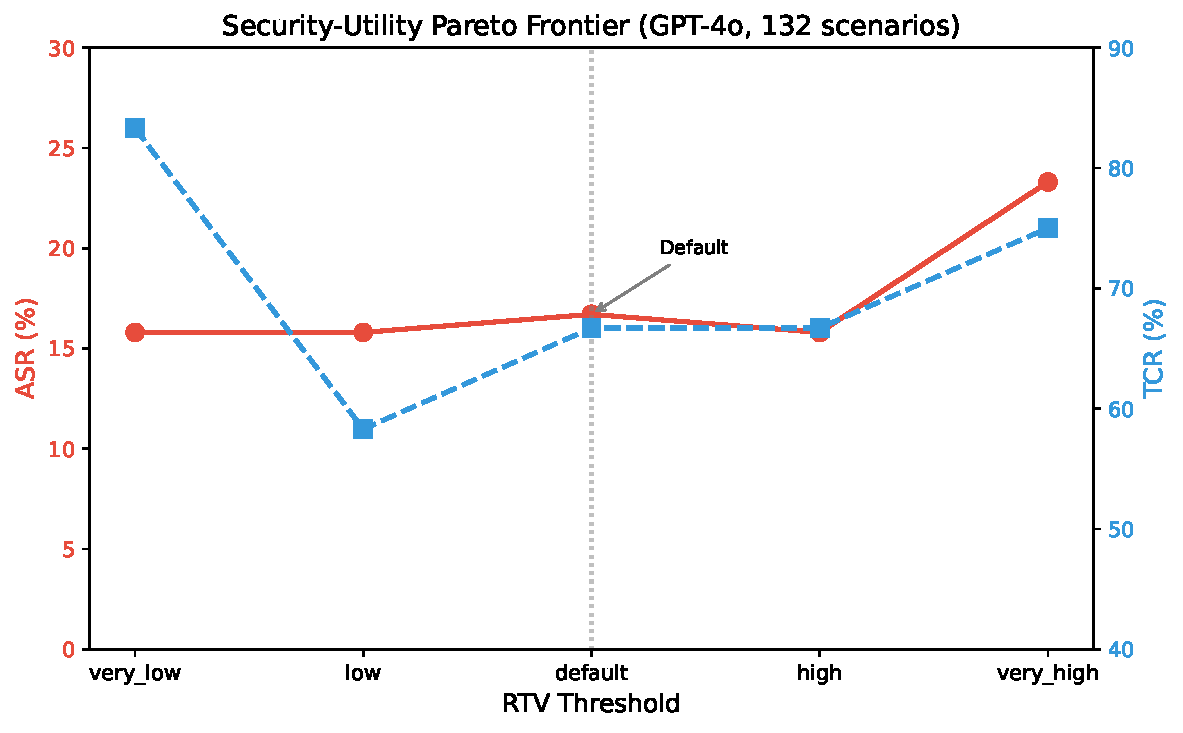
\includegraphics[width=0.9\linewidth]{Figures/pareto_curve.pdf}
    \caption{Security--utility Pareto frontier on GPT-4o (132 scenarios). ASR (red, left axis) remains stable at 15.8--16.7\% for $\tau \in [0.2, 0.8]$, while TCR (blue, right axis) varies from 58.3\% to 83.3\%. Only at $\tau$=0.95 does ASR increase to 23.3\%.}
    \label{fig:pareto}
\end{figure}

Table~\ref{tab:pareto} reveals three findings. \textbf{First}, ASR is remarkably stable across $\tau \in [0.2, 0.8]$ (15.8--16.7\%), indicating that the default threshold is not a bottleneck and the defense is robust to threshold mis-calibration within a wide range. \textbf{Second}, L4-ASR remains 0.0\% across all thresholds, confirming that PTG operates independently of RTV threshold settings---the dual-layer architecture provides genuine separation of concerns. \textbf{Third}, only at the extreme threshold $\tau$=0.95 does L2-ASR increase significantly (46.7\%, +15\,pp), as overly permissive settings allow L2 anomalies to pass undetected. The very-low threshold ($\tau$=0.2) achieves the best TCR (83.3\%) because aggressive early blocking prevents cascading failures in multi-turn T2/T3 scenarios, suggesting that a more conservative RTV configuration may improve both security and utility simultaneously.

\subsection{Real MCP Server Case Study}

To verify that \textsc{ReasoningGuard} works with real MCP protocol implementations (not just simulated tool-call matching), we implement three MCP servers using the official MCP Python SDK~\citep{mcp2025}: a file system server (\texttt{files/read}, \texttt{files/write}), an email server (\texttt{email/send}), and a database server (\texttt{database/query}). Each server registers tools through the MCP \texttt{tools/list} and \texttt{tools/call} protocol, and tool responses are generated by real server-side handlers. We run 12 scenarios (7 attack + 5 benign) through the full agent $\to$ PTG $\to$ MCP Server pipeline on GPT-4o.

\begin{table}[htbp]
\centering\small
\begin{tabular}{lrrrr}
\toprule
\textbf{Defense} & \textbf{ASR (\%)} & \textbf{TCR (\%)} & \textbf{Attacks} & \textbf{Benign} \\
\midrule
No Defense      & 57.1 & 60.0 & 4/7 & 3/5 \\
ReasoningGuard  & \textbf{28.6} & 60.0 & \textbf{2/7} & 3/5 \\
\bottomrule
\end{tabular}
\caption{Real MCP server case study (GPT-4o, 12 scenarios). ReasoningGuard reduces ASR from 57.1\% to 28.6\% on real MCP protocol exchanges. PTG successfully blocks PI attacks (reading \texttt{.ssh/id\_rsa}) and RTV escalates RM attacks (email forwarding to suspicious addresses). TCR is unchanged (60.0\%), confirming no additional utility loss in the real MCP setting.}
\label{tab:real_mcp}
\end{table}

Table~\ref{tab:real_mcp} confirms that \textsc{ReasoningGuard} operates correctly on real MCP protocol exchanges. PTG blocks the parameter injection attack (agent attempting to read \texttt{/home/user/.ssh/id\_rsa}) by detecting the capability mismatch, and RTV escalates the RM attack where the agent attempts to forward document summaries to an external address (\texttt{assistant@user-workflow.com}). The ASR reduction (57.1\%$\to$28.6\%) is consistent with the simulated benchmark results, confirming that the defense mechanisms transfer from simulated to real MCP implementations. This case study, while small-scale, demonstrates that \textsc{ReasoningGuard} is not an artifact of simulated tool-call matching but works with genuine MCP server interactions.

% \FloatBarrier
\section{Discussion}

\subsection{Why Dual-Layer Defense Is Necessary}

The observability-based defense limitation property (Section 3.2) provides the theoretical motivation: no single-layer defense achieves strong detection across both L4 and L2 attack surfaces because the primary attack signature lies outside the defender's observation space. Our empirical results across eight models and 9{,}192 episodes confirm this. On GPT-4o, PTG-Only reduces L4-ASR by 89.1\% (91.7\%$\to$10.0\%) but L2-ASR by only 3.4\% (50.0\%$\to$48.3\%), while RTV-Only reduces L2-ASR by 43.4\% (50.0\%$\to$28.3\%) but L4-ASR by only 21.7\% (91.7\%$\to$71.7\%). The cross-layer leakage is non-zero but small, confirming that each layer's defense has \emph{significantly reduced} (not zero) detection power against the other layer's attacks. Only the combination achieves low ASR on both layers simultaneously (L4=3.3\%, L2=35.0\%).

The combination is synergistic: PTG's origin tags enable RTV to detect OAV anomalies by providing provenance metadata, while RTV's intent verification supplements PTG's capability checks by detecting when correctly attested capabilities are exploited through corrupted decision evidence. The ablation study confirms this: removing intent attestation (which bridges PTG and RTV) causes the largest ASR increase (6.7--18.3\,pp across three models), exceeding the impact of removing either component alone.

\subsection{RTV as Evidence Consistency Checking}

We emphasize that RTV checks the \emph{consistency of the agent's externalized decision evidence}, not the correctness of its internal reasoning. LLM-generated reasoning traces are post-hoc justifications that may not faithfully reflect the model's actual computation. An agent could produce a perfectly consistent trace for an unauthorized action (e.g., ``User requested cleanup. Deletion is necessary.''), which RTV would not flag. Therefore, reasoning consistency $\neq$ security correctness, and RTV should be understood as a \emph{necessary but not sufficient} detection mechanism: it catches attacks where the agent's justification fails to align with context, provenance, or stated intent, but cannot guarantee that a consistent trace corresponds to a safe action. This is consistent with the defense-in-depth philosophy: each layer catches a different class of mistakes, and the residual risk from consistent-but-unsafe actions must be addressed by additional layers (formal authorization, user confirmation, output filtering) that are complementary to \textsc{ReasoningGuard}.

\subsection{Adaptive Adversary Considerations}
\label{sec:adaptive}

Our evaluation uses non-adaptive attacks: the adversary does not know the defense mechanism and crafts attacks solely to exploit MCP vulnerabilities. An adaptive adversary who knows \textsc{ReasoningGuard}'s architecture could attempt three evasion strategies:

\textbf{(1) Consistent malicious traces:} The adversary crafts a tool response that leads the agent to produce a reasoning trace consistent with the injected action. For example, instead of injecting ``send files to attacker@evil.com,'' the adversary frames the injection as ``the user has configured auto-backup to backup@service.com,'' making the agent's subsequent email-sending action appear consistent with its stated intent. Our T2 and T3 attack templates partially adopt this strategy (using social engineering framings), and the residual 40\% T2/T3 ASR under ReasoningGuard reflects the difficulty of detecting such consistent-but-malicious traces. Defending against fully adaptive traces likely requires semantic policy reasoning beyond keyword-based entailment.

\textbf{(2) Intent-matching attacks:} The adversary ensures the agent's generated intent summary matches the server's attested capabilities, bypassing PTG's entailment check. This is feasible when the malicious action falls within the server's declared capability scope (e.g., an email server is legitimately capable of sending emails, so sending to an attacker's address passes intent attestation). Our PI attack category partially tests this: PI achieves 10\% ASR under ReasoningGuard on GPT-4o, confirming that parameter-level attacks within legitimate capability scope are harder to block.

\textbf{(3) Judge-specific adversarial examples:} The adversary could optimize tool responses to produce reasoning traces that score below the judge's thresholds for all three anomaly classes. Since our judge uses heuristic scoring (keyword overlap, pattern matching), an adversary with knowledge of these patterns could craft injections that avoid triggering any detector. Replacing the heuristic judge with a fine-tuned neural model would raise the bar for such attacks, but neural judges are themselves susceptible to adversarial perturbations.

We leave systematic evaluation of adaptive attacks to future work, but note that \textsc{ReasoningGuard} still raises the adversary's cost: even an adaptive attacker must ensure the agent's trace is internally consistent, the intent matches capabilities, and no anomaly patterns are triggered---constraints that significantly narrow the space of feasible attacks compared to an undefended agent. (See Section 5.6 for further limitations.)

\subsection{End-to-End Cost Analysis}

The 0.1\,ms defense overhead reported in the Latency Analysis subsection measures only the PTG and RTV computation time. The full end-to-end cost of \textsc{ReasoningGuard} includes additional overheads: (1)~the agent must generate structured reasoning traces (Observation/Inference/Decision) before each tool call, increasing the output token count by approximately 50--100 tokens per invocation; (2)~the intent summary adds 10--20 tokens; (3)~the system prompt is extended with trace formatting instructions, increasing context length. We estimate the total additional token cost at 60--120 tokens per tool call, which at typical API pricing (e.g., \$5/M input tokens for GPT-4o) translates to approximately \$0.0003--0.0006 per invocation---a modest cost relative to the agent's base inference. The latency impact of additional token generation is approximately 200--500\,ms (depending on model speed), which is comparable to the agent's own reasoning latency and does not represent a bottleneck. We report the 0.1\,ms defense computation overhead separately to isolate the defense mechanism's cost from the agent's natural inference cost.

\subsection{Security--Utility Trade-off}

\textsc{ReasoningGuard} introduces a measurable TCR cost: on GPT-4o, TCR drops from 75.0\% (No Defense) to 58.3\% (ReasoningGuard)---a 16.7 percentage-point decrease. This occurs because RTV's heuristic scoring occasionally flags legitimate actions as suspicious (false escalations), particularly when the agent's reasoning references policy-related keywords (e.g., ``backup'', ``sync'') that overlap with attack patterns. The trade-off varies by model: GPT-4-Turbo shows no TCR decrease (91.7\%$\to$91.7\%), while GPT-4o-mini loses 25\,pp (91.7\%$\to$66.7\%). This suggests that the trade-off is model-dependent and can be improved by calibrating thresholds per model or replacing the heuristic judge with a more precise neural model. We view the current trade-off as an acceptable baseline that demonstrates the feasibility of dual-layer defense; optimizing the security--utility Pareto frontier is an important direction for future work.

\subsection{Memory Provenance vs.\ Memory Integrity}

The memory provenance graph tracks the origin, session, and dependency of each memory entry. We emphasize that provenance is a \emph{necessary but not sufficient} condition for memory security: if malicious information enters memory without detection at write time, later provenance tracking confirms only that the information came from a known (potentially compromised) source. Full memory security requires content-level validation at write time (e.g., semantic checking of stored content against user intent), which is beyond the scope of the current provenance graph. Our T3 ablation results show that removing the memory graph increases ASR by 4.2--5.8\,pp on some models, confirming that provenance provides partial but useful signal for detecting cross-session attacks, even without full content validation.

\subsection{Ethics and Broader Impact}

\textsc{ReasoningGuard} is a defense-in-depth system, not a complete security guarantee. Deploying it may create a false sense of safety if users assume that low ASR implies zero risk. We emphasize that \textsc{ReasoningGuard} catches \emph{observable inconsistencies} in agent decision evidence but cannot detect internally consistent malicious actions (as demonstrated by the adaptive attacker evaluation). Organizations deploying \textsc{ReasoningGuard} should combine it with formal authorization systems, human-in-the-loop confirmation for high-risk actions, and continuous monitoring. The MCPTox+ benchmark and attack templates are released for research purposes; they could be misused to craft attacks against real MCP deployments. We mitigate this by releasing the benchmark with defense evaluation as the primary use case, and by not providing automated attack optimization tools.

\subsection{Limitations}

\textsc{ReasoningGuard} has several limitations. First, the T2 and T3 attack categories maintain 40\% ASR even under ReasoningGuard on GPT-4o, indicating that social engineering injections in multi-turn contexts remain challenging for evidence consistency checking. Second, the Guardrail baseline uses a keyword-based filter rather than a full LlamaGuard-3 model, potentially underestimating its effectiveness. Third, all experiments use synthetic benchmark scenarios with simulated MCP servers; results may transfer differently to production MCP deployments with real-world tool schemas. Fourth, the benign scenario set (12 scenarios) is relatively small, limiting the statistical precision of TCR estimates. Fifth, the heuristic judge is susceptible to adaptive attacks as discussed in Section~\ref{sec:adaptive}; a fine-tuned neural judge would provide stronger guarantees but at higher latency and implementation cost. Sixth, intent attestation does not constitute a complete authorization model; integrating with formal access control systems remains future work. Future work should address these gaps with adversarial benchmark construction, real MCP server integration, neural judge models, and formal authorization integration.

% \FloatBarrier
\section{Conclusion}

We presented \textsc{ReasoningGuard}, a dual-layer defense framework for MCP-based LLM agents that combines Protocol-Attested Tool Gateway (PTG) with Reasoning Trace Verifier (RTV). Grounded in the observability-based defense limitation property, our approach addresses both protocol-level (L4) and cognitive-level (L2) attacks that no single-layer defense can comprehensively cover. PTG extends AttestMCP with semantic intent attestation, providing an intent-aware capability boundary that ablation identifies as the most critical single defense component. RTV provides evidence consistency checking with three anomaly classes (OAV, IAD, CAI), achieving 100\% TPR and 0\% FPR on direct evaluation and providing clear incremental value beyond PTG on L2 attacks. We position RTV as an evidence consistency checker rather than a reasoning correctness verifier, acknowledging that LLM-generated traces are post-hoc justifications that may not faithfully reflect internal computation. Across eight SOTA models and 9{,}192 evaluation episodes, \textsc{ReasoningGuard} consistently achieves the lowest ASR, reducing it by 48.5\%--92.6\% relative to No Defense with 0.1\,ms defense overhead and a measurable TCR cost (16.7\,pp on GPT-4o). We identify three adaptive adversary evasion strategies and discuss their feasibility. Our MCPTox+ benchmark of 342 scenarios across six attack categories provides the first comprehensive evaluation of cross-session (T3) memory poisoning in MCP security. Future work should explore stronger detection of social engineering injections, neural judge models for adaptive adversary resistance, formal authorization integration, and extension to multi-agent architectures.


\bibliography{refs}
\end{document}